\newif\ifshowsolutions
\showsolutionsfalse
\documentclass{article}
\usepackage{listings}
\usepackage{amsmath}
%\usepackage{subfigure}
\usepackage{subfig}
\usepackage{amsthm}
\usepackage{amsmath}
\usepackage{amssymb}
\usepackage{graphicx}
\usepackage{mdwlist}
\usepackage[colorlinks=true]{hyperref}
\usepackage{geometry}
\usepackage{titlesec}
\geometry{margin=1in}
\geometry{headheight=2in}
\geometry{top=2in}
\usepackage{palatino}
\usepackage{mathrsfs}
\usepackage{fancyhdr}
\usepackage{paralist}
\usepackage{todonotes}
\setlength{\marginparwidth}{2.15cm}
\usepackage{tikz}
\usetikzlibrary{positioning,shapes,backgrounds}
\usepackage{float} % Place figures where you ACTUALLY want it
\usepackage{comment} % a hack to toggle sections
\usepackage{ifthen}
\usepackage{mdframed}
\usepackage{verbatim}
\usepackage[strings]{underscore}
\usepackage{listings}
\usepackage{bbm}
\usepackage{poemscol}
\rhead{}
\lhead{}

\fancyfoot[C]{\thepage}
\renewcommand{\baselinestretch}{1.15}

% Shortcuts for commonly used operators
\newcommand{\E}{\mathbb{E}}
\newcommand{\Var}{\operatorname{Var}}
\newcommand{\Cov}{\operatorname{Cov}}
\newcommand{\Bias}{\operatorname{Bias}}
\DeclareMathOperator{\argmin}{arg\,min}
\DeclareMathOperator{\argmax}{arg\,max}

% do not number subsection and below
\setcounter{secnumdepth}{1}

% custom format subsection
\titleformat*{\subsection}{\large\bfseries}

% set up the \question shortcut
\newcounter{question}[section]
\newenvironment{question}[1][]
  {\refstepcounter{question}\par\addvspace{1em}\textbf{Question~\Alph{question}\!
    \ifthenelse{\equal{#1}{}}{}{ [#1 points]}: }}
    {\par\vspace{\baselineskip}}

\newcounter{subquestion}[question]
\newenvironment{subquestion}[1][]
  {\refstepcounter{subquestion}\par\medskip\textbf{\roman{subquestion}.\!
    \ifthenelse{\equal{#1}{}}{}{ [#1 points]:}} }
  {\par\addvspace{\baselineskip}}

\titlespacing\section{0pt}{12pt plus 2pt minus 2pt}{0pt plus 2pt minus 2pt}
\titlespacing\subsection{0pt}{12pt plus 4pt minus 2pt}{0pt plus 2pt minus 2pt}
\titlespacing\subsubsection{0pt}{12pt plus 4pt minus 2pt}{0pt plus 2pt minus 2pt}


\newenvironment{hint}[1][]
  {\begin{em}\textbf{Hint: }}{\end{em}}

\if showsolutions
  \newenvironment{solution}[1][]
    {\par\medskip \begin{mdframed}\textbf{Solution~\Alph{question}#1:} \begin{em}}
    {\end{em}\medskip\end{mdframed}\medskip}
  \newenvironment{subsolution}[1][]
    {\par\medskip \begin{mdframed}\textbf{Solution~\Alph{question}#1.\roman{subquestion}:} \begin{em}}
    {\end{em}\medskip\end{mdframed}\medskip}
\else
  \excludecomment{solution}
  \excludecomment{subsolution}
\fi

\renewcommand{\headrulewidth}{0.4pt}
\graphicspath{{../output/}}

\chead{%
  {\vbox{%
      \vspace{2mm}
      \large
      Machine Learning \& Data Mining \hfill
      Caltech CS/CNS/EE 155 \hfill \\[1pt]
      Miniproject 3\hfill
      \today\\
      Richard Cheng, Yoke Peng Leong, Daniel Pastor
    }
  }
}

\begin{document}
\pagestyle{fancy}
\section{Basic Visualization}

Figure \ref{fig:all-movie} shows the visualization of the average ratings for all movies in the MovieLens dataset. A histogram of the average ratings provide an overview of the distribution of the ratings of all movies. We can observe that most movies have an average rating between 3 and 3.5. 

\begin{figure}[H]
	\centering
	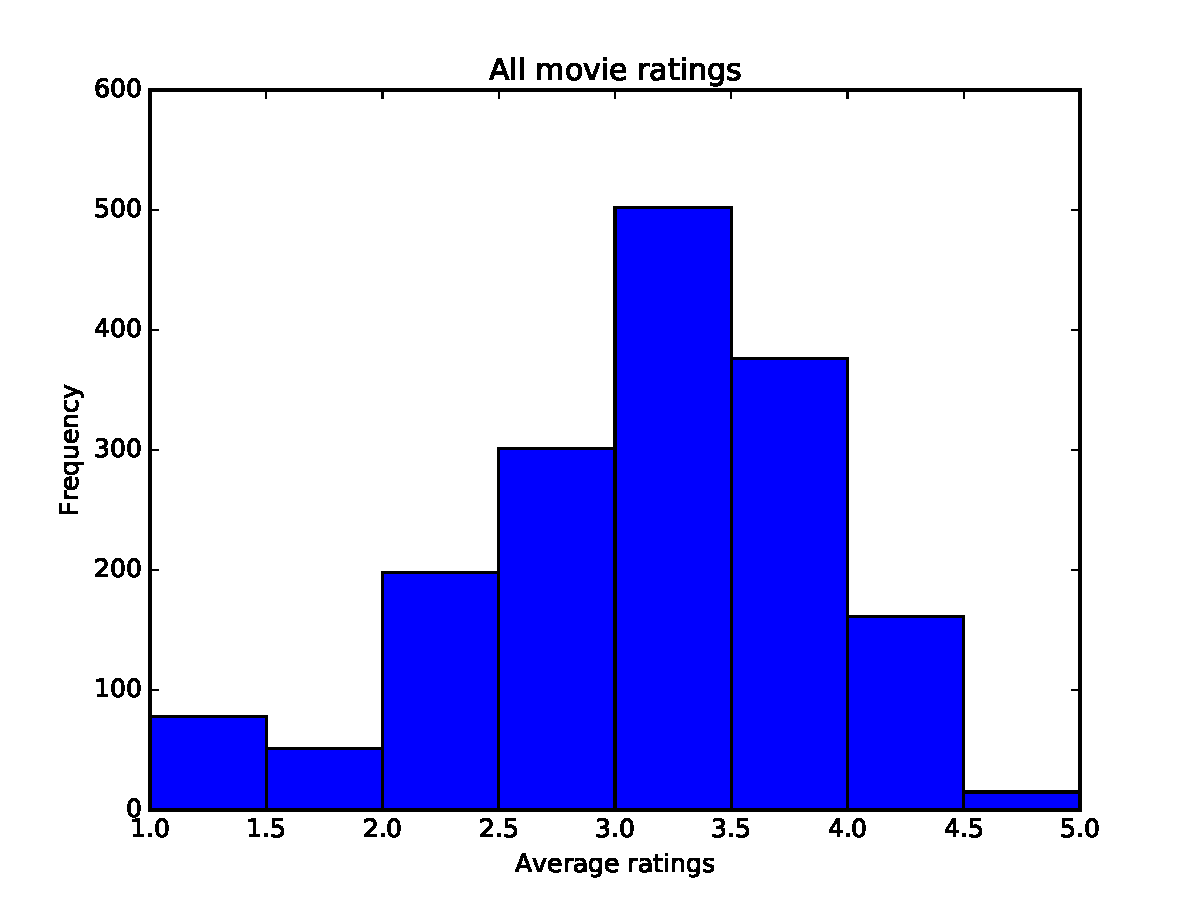
\includegraphics[width=\textwidth]{all_movie_ratings}
	\caption{Average ratings for all movies in MovieLens.} \label{fig:all-movie}
\end{figure}


Figure \ref{fig:all-movie-sorted} provides another view of the average ratings for all movie in the MovieLens dataset. We can observe that when the average ratings are integers, there are small numbers of ratings, indicating that the average ratings at those integer values may not be reliable.

\begin{figure}[H]
	\centering
	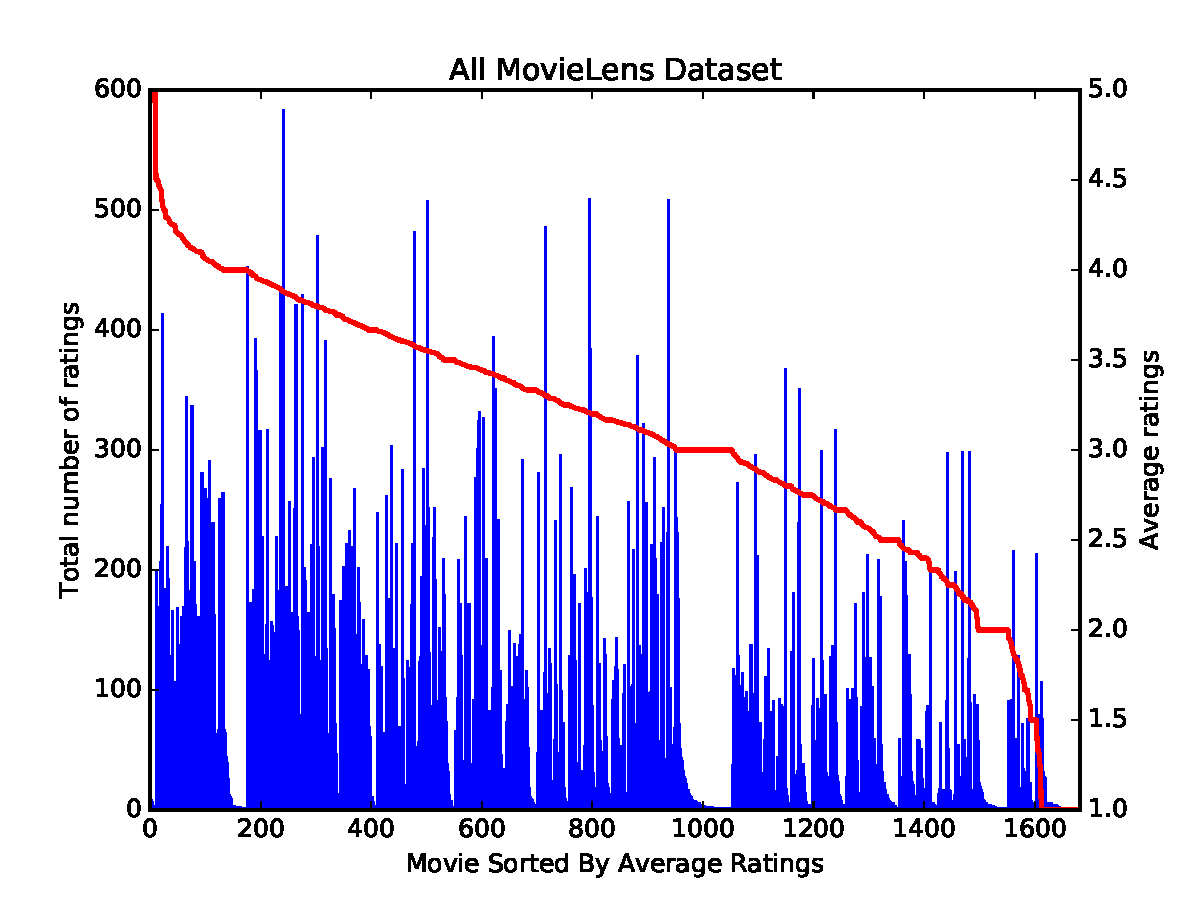
\includegraphics[width=\textwidth]{sorted_ratings}
	\caption{Average ratings for all movies in MovieLens sorted according to the average ratings. Red line represents the average ratings, and blue bars represent the total number of ratings.} \label{fig:all-movie-sorted} 
\end{figure}

Figures \ref{fig:top-10-best} and \ref{fig:top-10-popular} show distribution of ratings for the top 10 best movies and top 10 most popular movies respectively. First, we can see that the top 10 best movies have small numbers of ratings, but they are all 5 resulting in average ratings of 5. This observation indicates that the ratings are not too reliable. Second, the top most popular movies tend to have high ratings. This observation indicates that a popular movie tends to be a good movie. It might also indicate that a good movie tends to be a popular movie. The causality is unclear, but good movies seem to be correlated to popular movies, making logical sense. 

\begin{figure}[H]
	\centering
	\subfloat[Top 10 best movies] {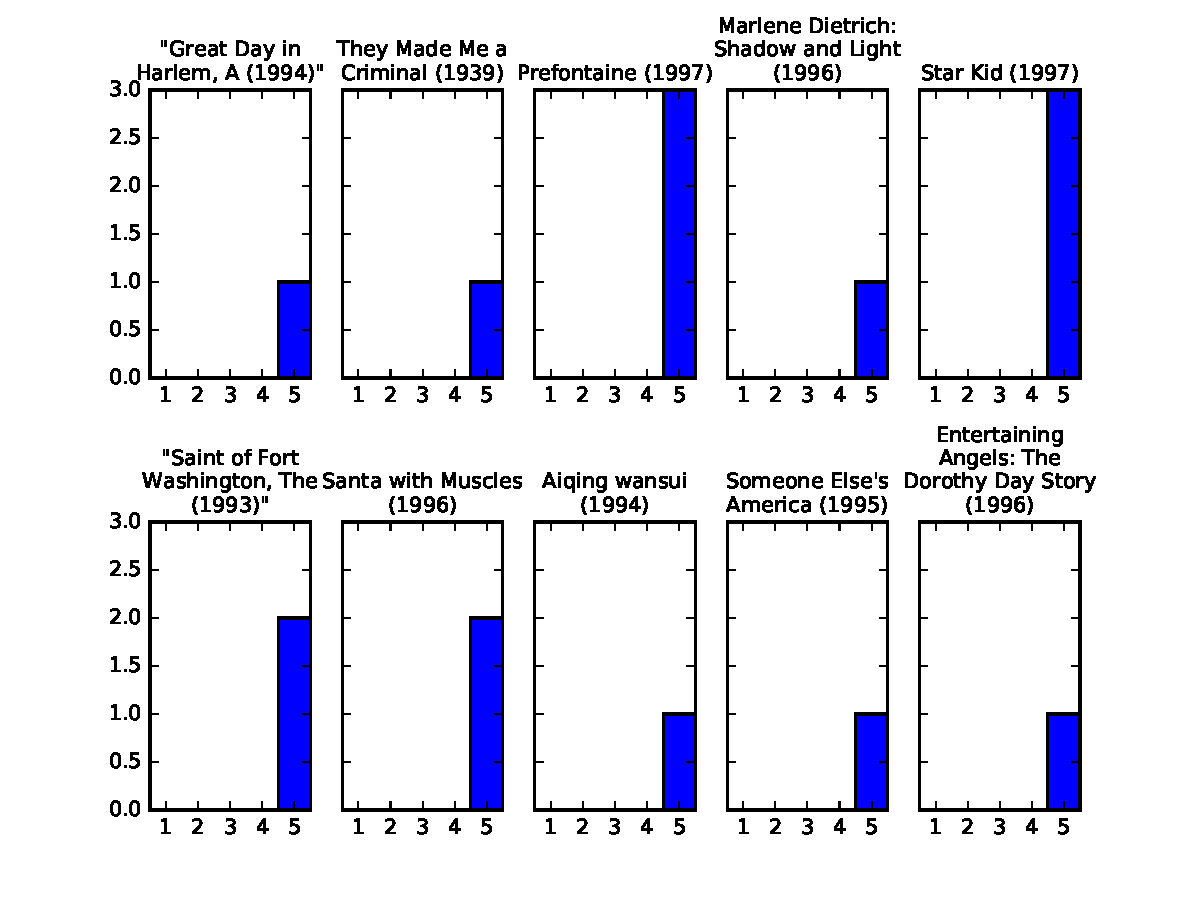
\includegraphics[width=0.8\textwidth, trim = 0cm 0mm 0cm 1cm, clip=true] {top_10_best_movie}\label{fig:top-10-best}}\\
	\subfloat[Top 10 most popular movies] {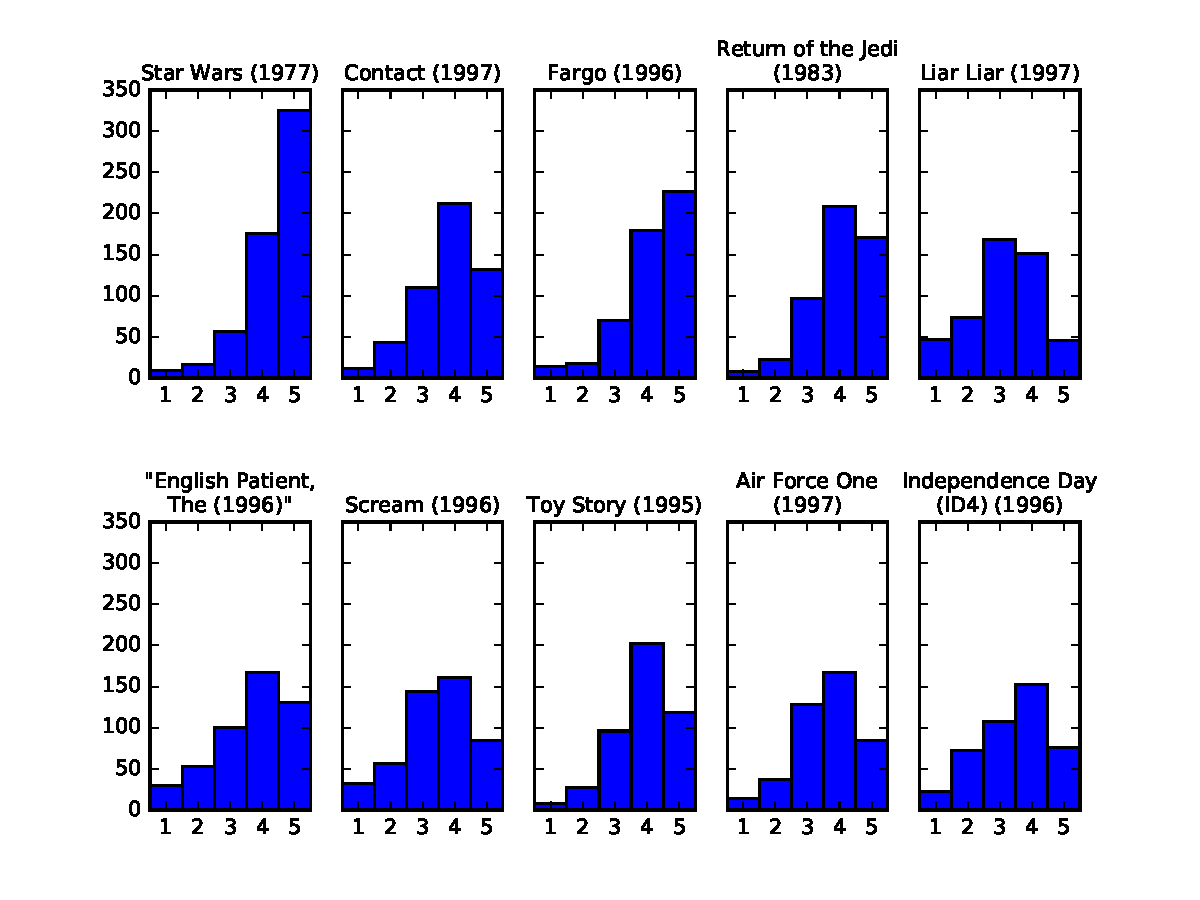
\includegraphics[width=0.8\textwidth, trim = 0cm 0mm 0cm 1.3cm, clip=true]{top_10_popular_movie}\label{fig:top-10-popular}}
	\caption{Ratings of top movies.} 
\end{figure}

Figure \ref{fig:average-3-genres} shows the average ratings of all movies in four different genres -- children, fantasy, horror, and documentary. There are fewer fantasy movies than children, horror, and documentary. The first three genres seem to have average ratings of about 2.5 to 3. The documentary genre has more high average ratings than the rest. In fact, the documentary genre seems to have more movies with above average ratings than movies with below average ratings. The other genres are more balanced. The documentary movies have a peak near average ratings of 3 to 3.5 and a small peak near average ratings of 1 to 1.5. This result indicates that documentaries are either really bad or good (above average ratings of 3).


\begin{figure}[H]
	\centering
	\subfloat[Children]{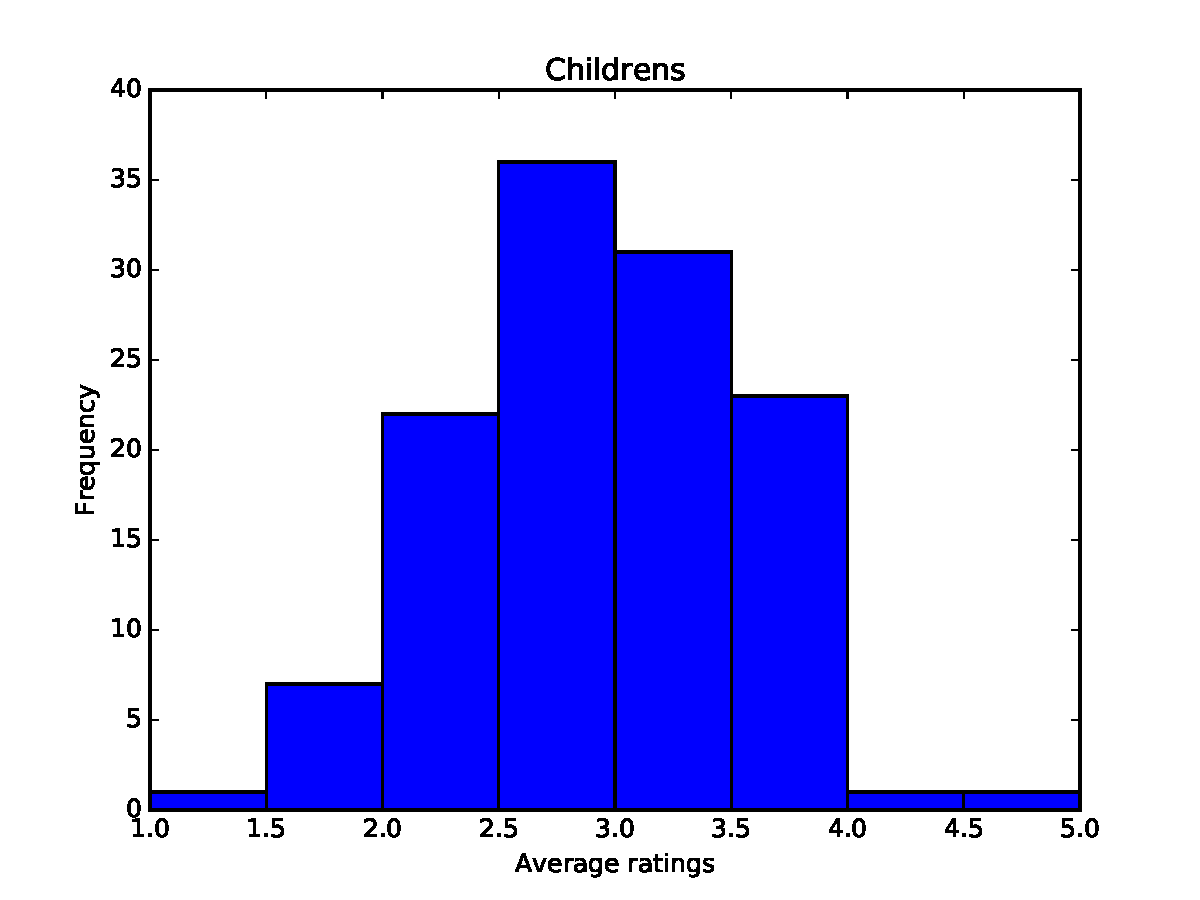
\includegraphics[width=0.45\textwidth, trim = 1cm 0mm 2cm 0mm, clip=true]{movie_genre_4}}
	\subfloat[Fantasy]{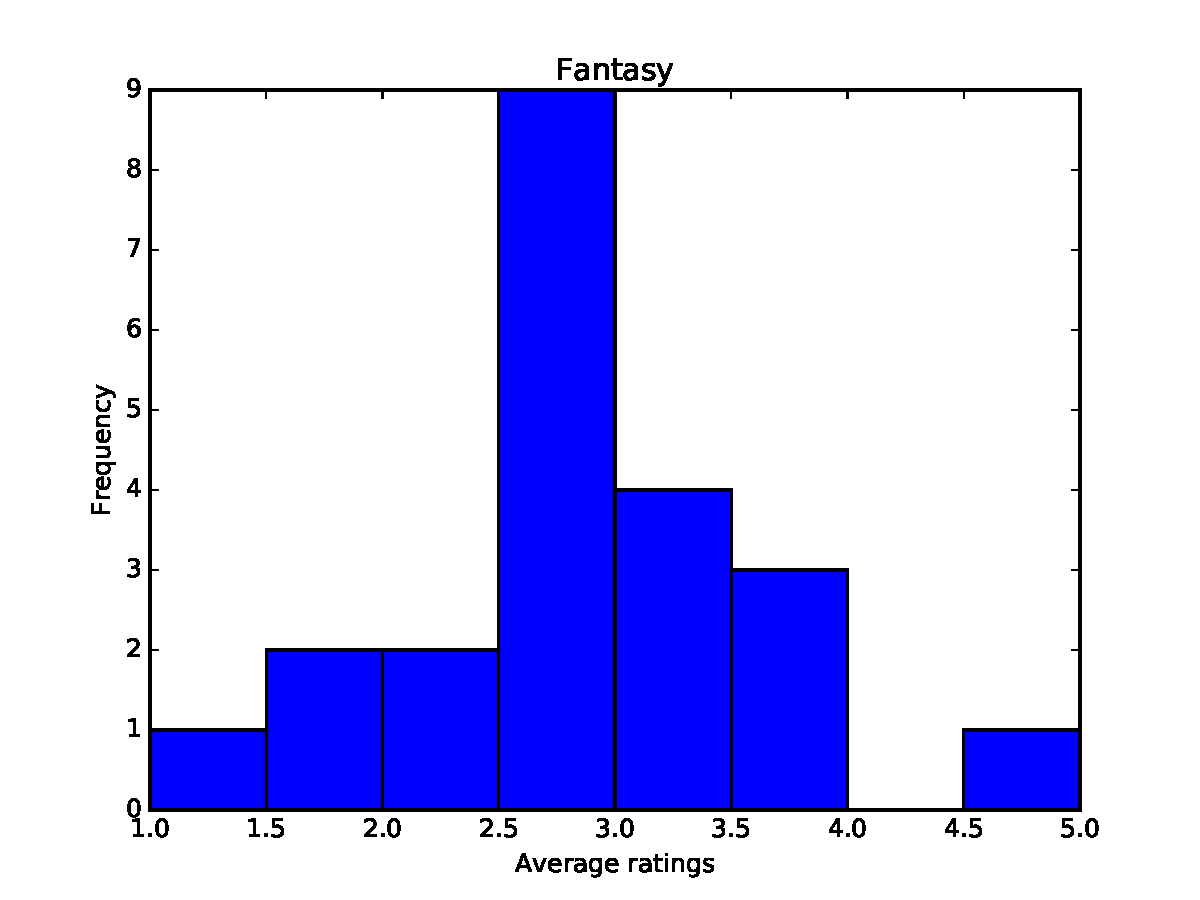
\includegraphics[width=0.45\textwidth, trim = 1cm 0mm 2cm 0mm, clip=true]{movie_genre_9}}\\
	\subfloat[Horror]{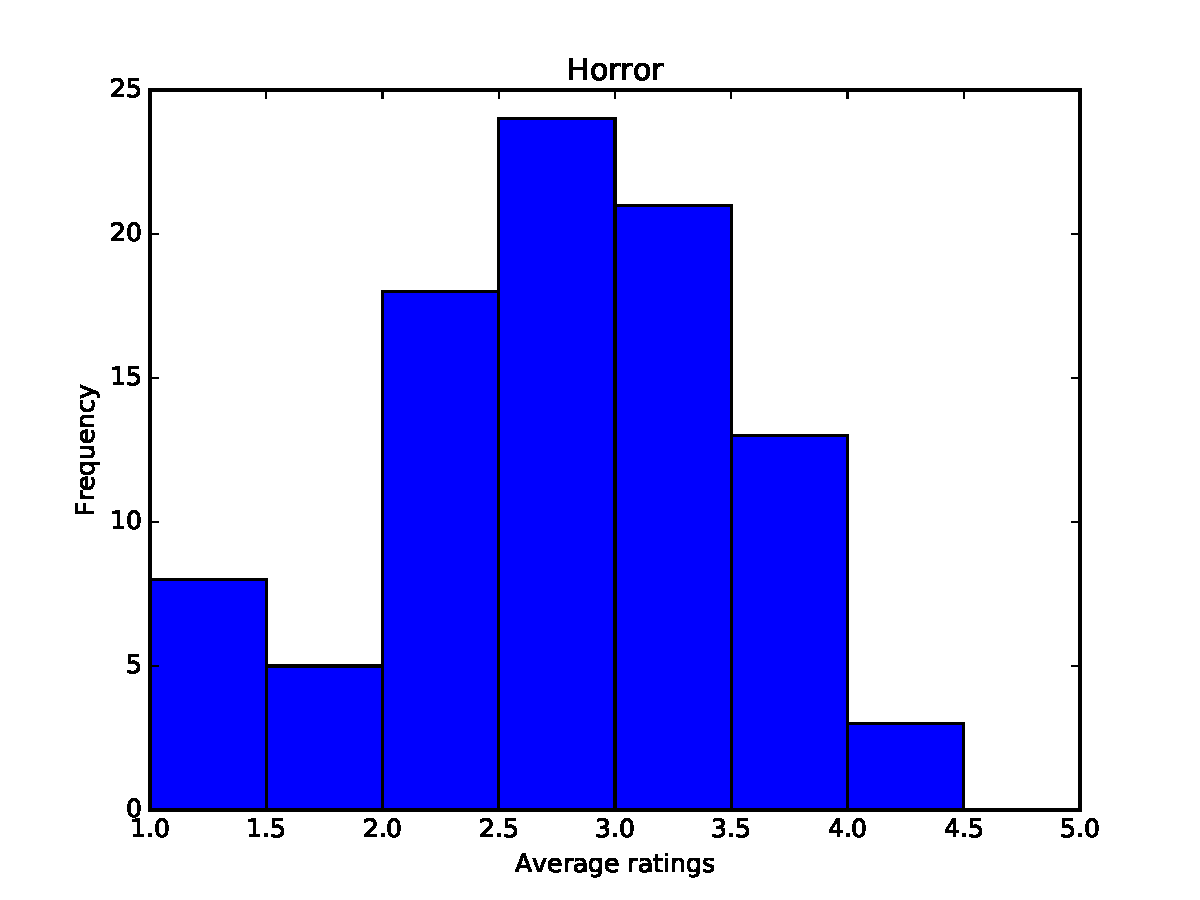
\includegraphics[width=0.45\textwidth, trim = 1cm 0mm 2cm 0mm, clip=true]{movie_genre_11}}
	\subfloat[Documentary]{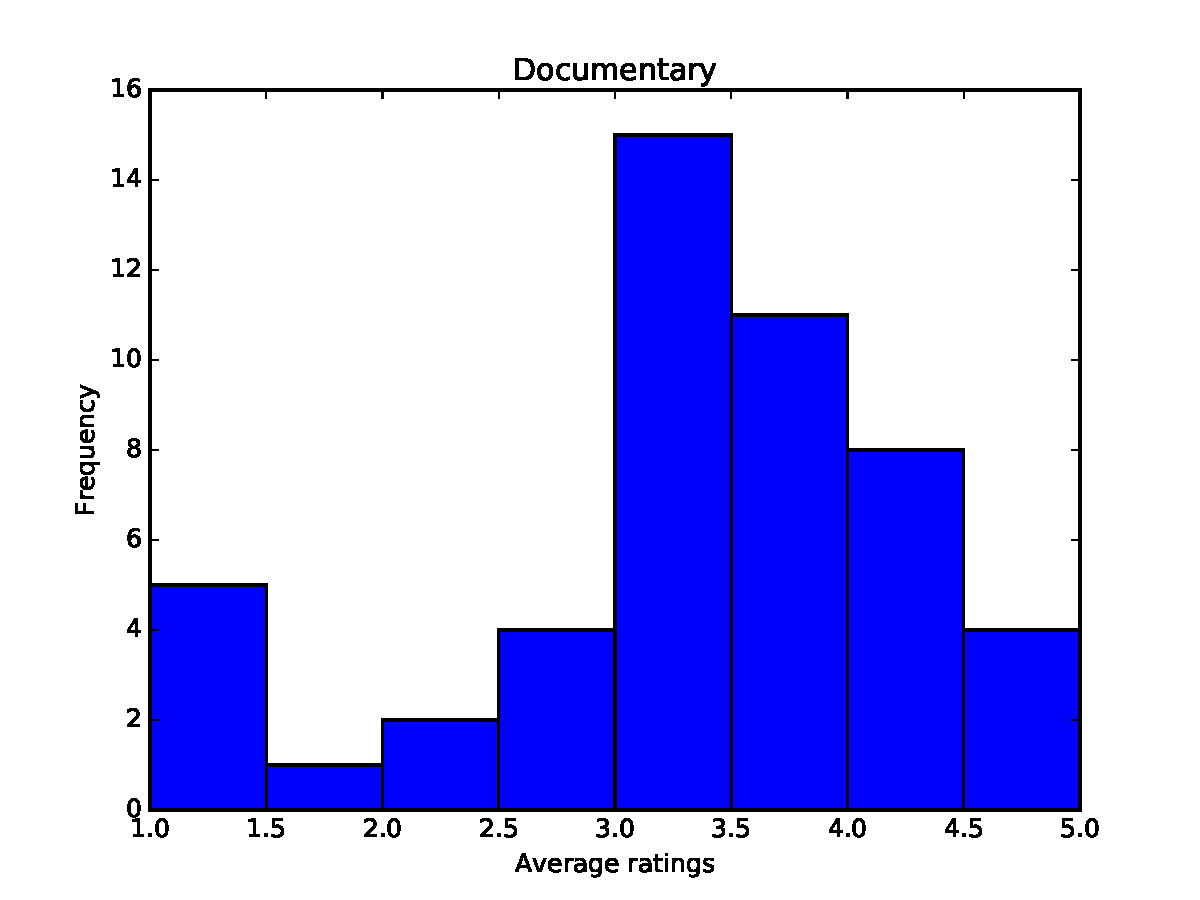
\includegraphics[width=0.45\textwidth, trim = 1cm 0mm 2cm 0mm, clip=true]{movie_genre_7}}
	\caption{Average ratings of all movies in four different genres.} \label{fig:average-3-genres}
\end{figure}

\section{Matrix Factorization Algorithm}

\medskip

\subsection{Training U and V}

~

We used the TA solution (prob2utils.py) to train $U$ and $V$  (matrix factorization of Y) to minimize the objective function:

$$\frac{\lambda}{2} ( ||U||_{Fro}^2 + ||V||_{Fro}^2) + \sum_{ij} (y_{ij} - u_i^T v_j)^2$$

We took the regularization parameter $\lambda = 0.01$, similar to what we used in HW \#6. The goal was to approximate $U$ and $V$ such that $Y \approx U V^T$. 

\subsection{Projecting U and V}

In order to visualize the resulting latent factors, we wanted to project $U$ and $V$ onto a two-dimensional space. The first thing we do though, is mean center $V$ and also shift $U$ accordingly.  This ensure that each row of $V$, representing a characteristic weighting of movies, is zero-centered and $U$ is consistently shifted with $V$. 

Then we applied an SVD to $U$ and $V$ so that $U = A_U \Sigma_U B_U^T$ and $V = A_V \Sigma_V B_V^T$. The first 2 columns of $A_V$ correspond to the best 2-dimensional projection of movies, and the first 2 columns of $A_U$ correspond to the best 2-dimensional projection of users.

Then $\tilde{V} = A_{V(1:2)}^T V$ projects the movies onto a 2-dimensional space representing the top 2 principal components of $V$ (the 2 dimensions that capture the most variance in movies). Also $\tilde{U} = A_{U(1:2)}^T U$ does the same thing for users rather than movies. Finally, we scaled each row of $\tilde{V}$ and $\tilde{U}$ to have unit variance so that the axes would not look too stretched.


\section{Matrix Factorization Visualization}

For each movie \textit{j} we visualize it as a 2D vector using the coordinates $\bar{V}[1:2,j]$, where $\bar{V}$ is obtained from the previous section. We show 10 random movies in Figure~\ref{fig:tenRandom}, the most popular 10 movies in Figure~\ref{fig:tenMostPopular} and the best 10 movies in Figure~\ref{fig:tenBest}. We observe that similar movies are closer together but in general there is no correlation between distance in the plots and movie similarity as seen by the authors. \\
The observe that the most popular 10 movies are located along the line $(1,1)$ while the best 10 movies cover the 2D space more uniformly .
Figure~\ref{fig:tg} shows the representation for the genres horror, children and fantasy. The movies withing each genre tend to cluster together but the variance for each genre is very high as it can be seen in .

\begin{figure}[hptb]
\centering
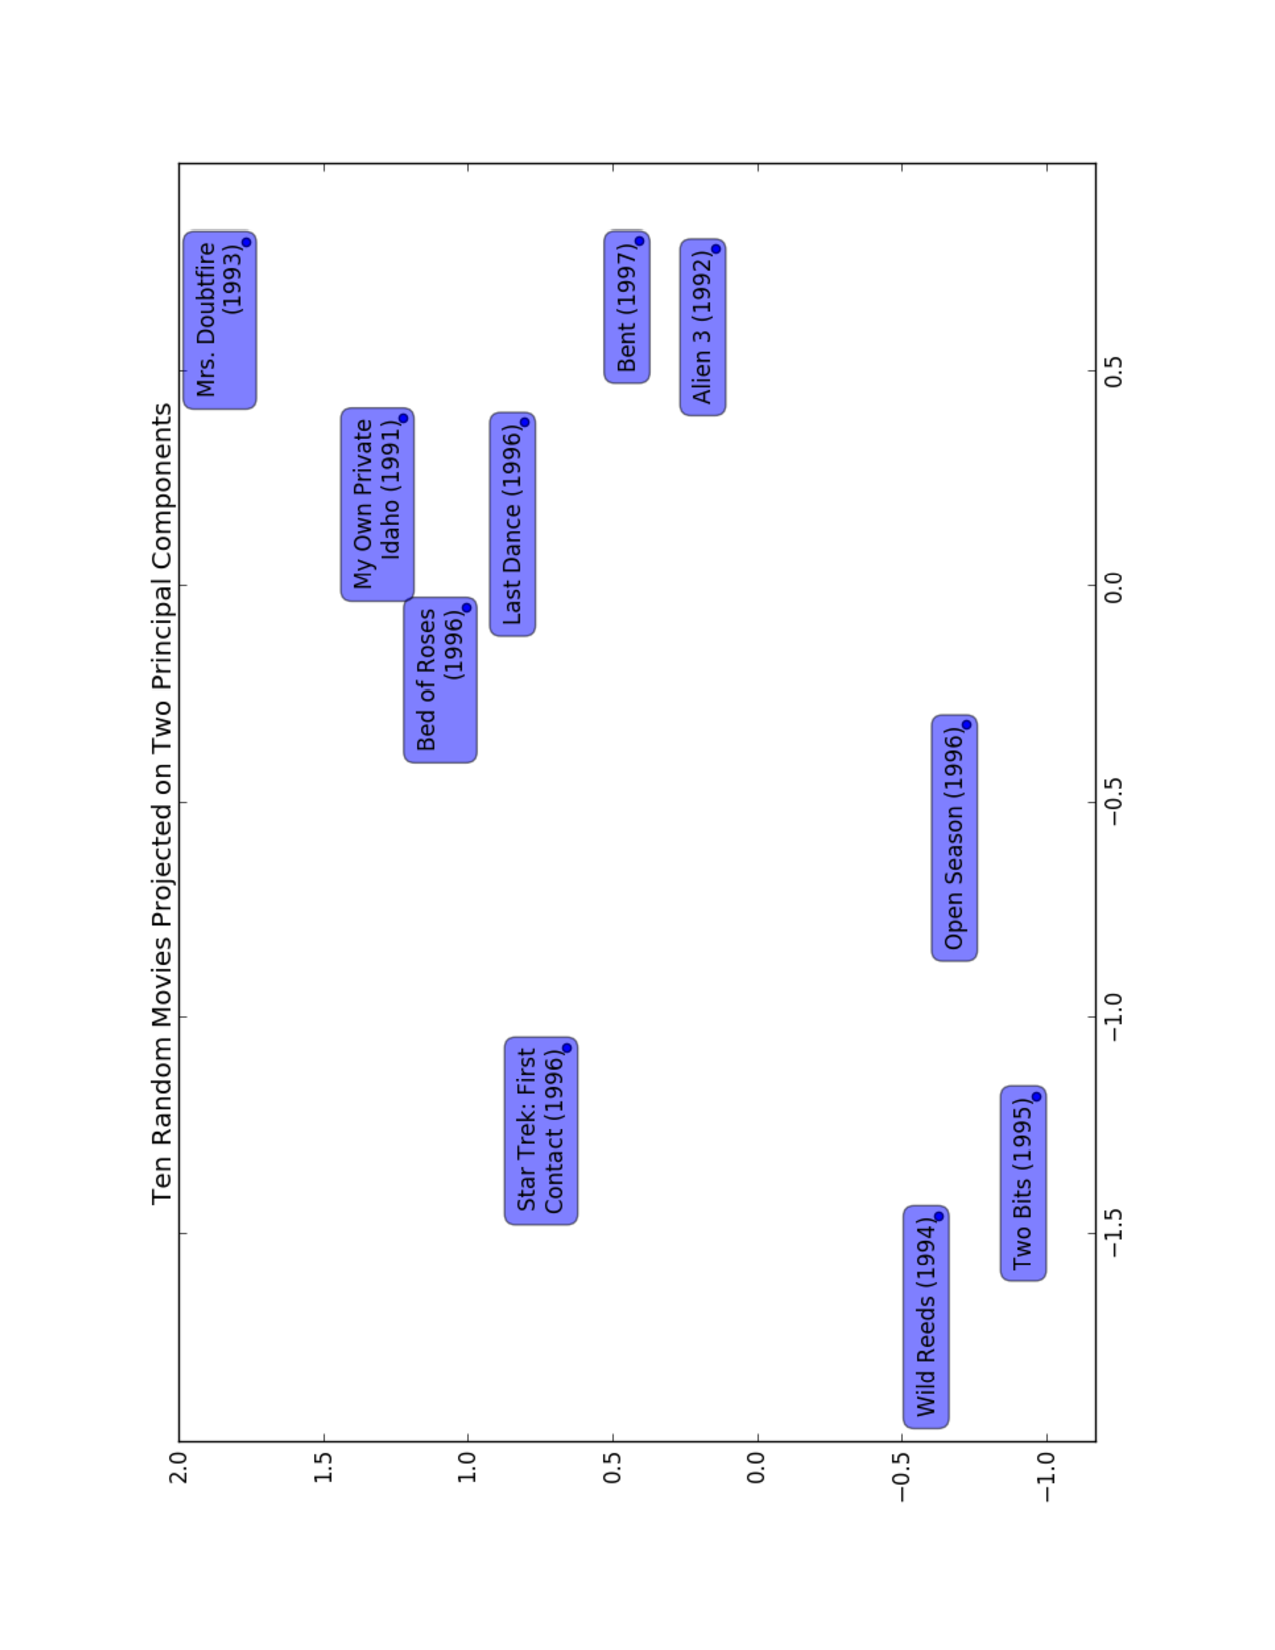
\includegraphics[width=0.8\textwidth, angle =270]{Random_10_Movies.pdf}
 \caption{Ten Random movies projected along two principal components.}
\label{fig:tenRandom}
\end{figure}


\begin{figure}[hptb]
\centering
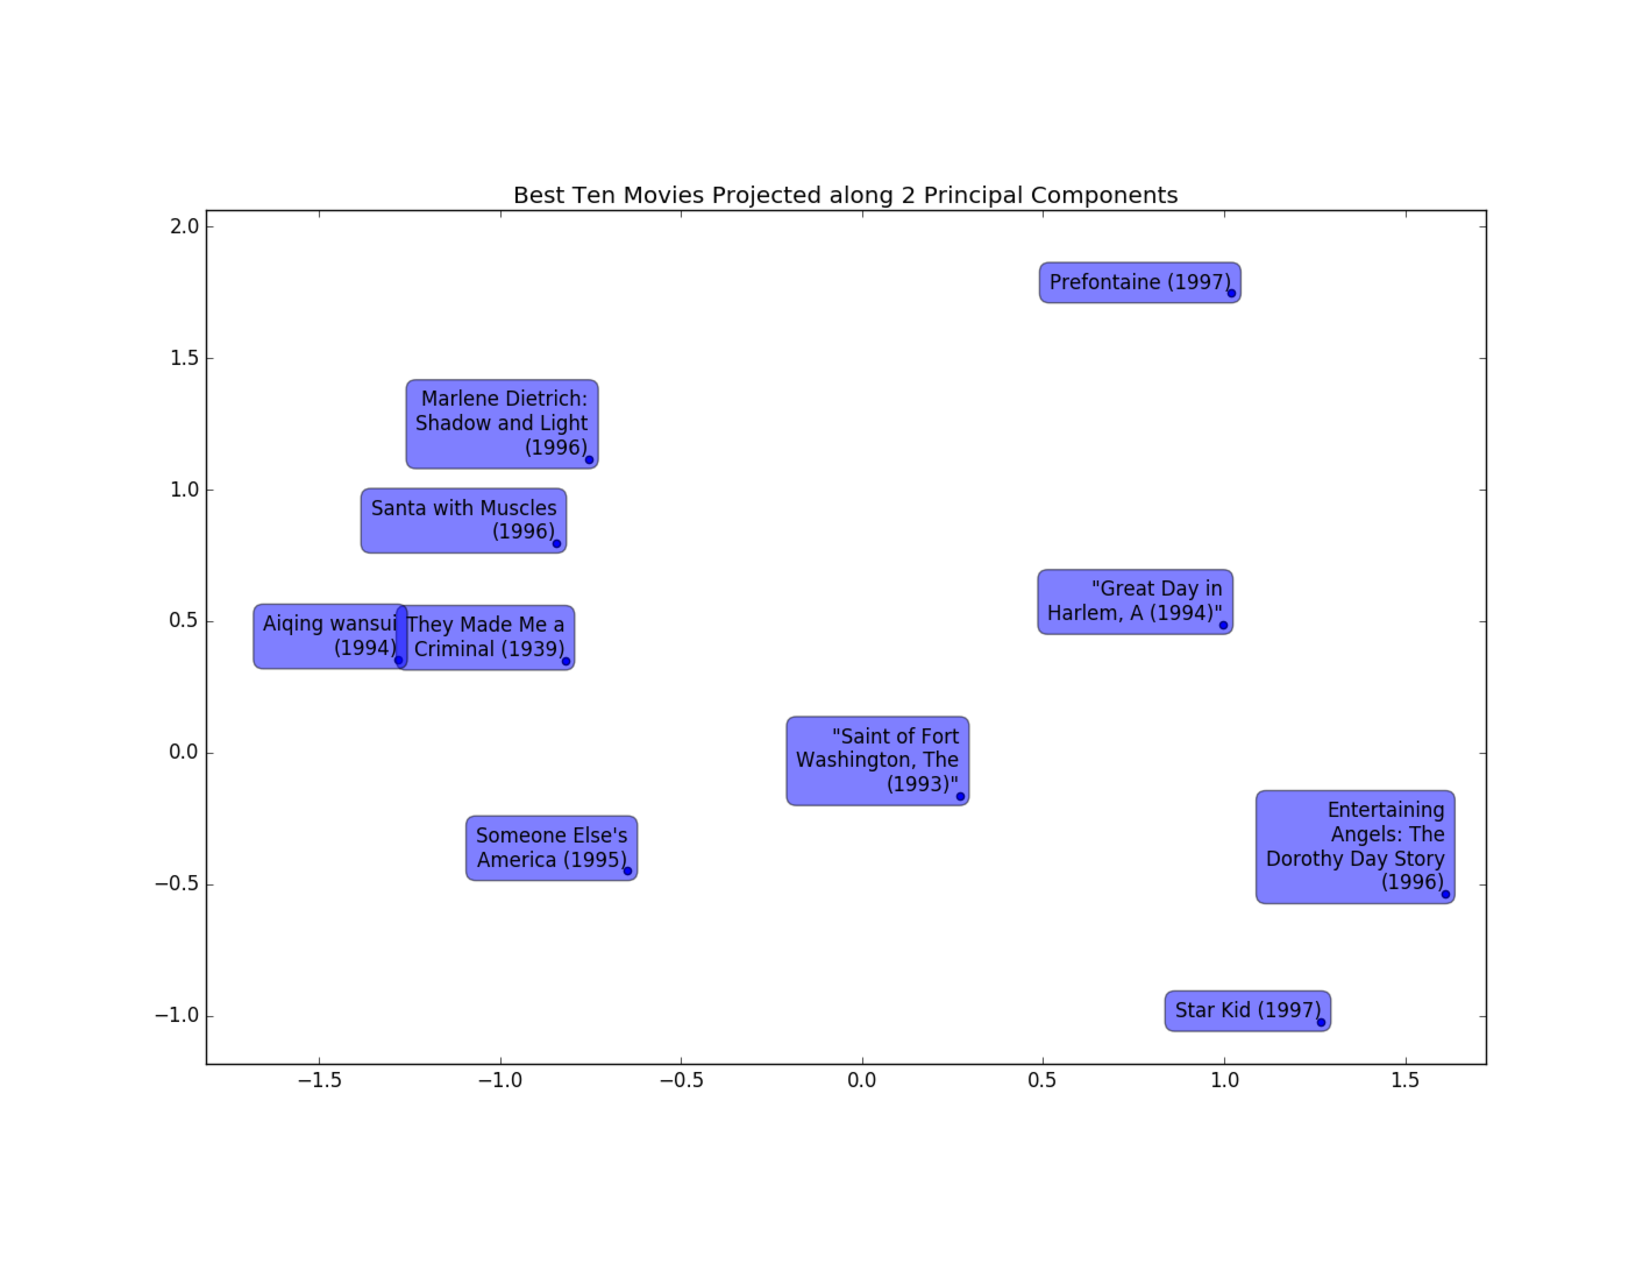
\includegraphics[width=0.8\textwidth, angle = 270]{Best_10_Movies.pdf}
 \caption{Best ten movies projected along two principal components.}
\label{fig:tenBest}
\end{figure}


\begin{figure}[hptb]
\centering
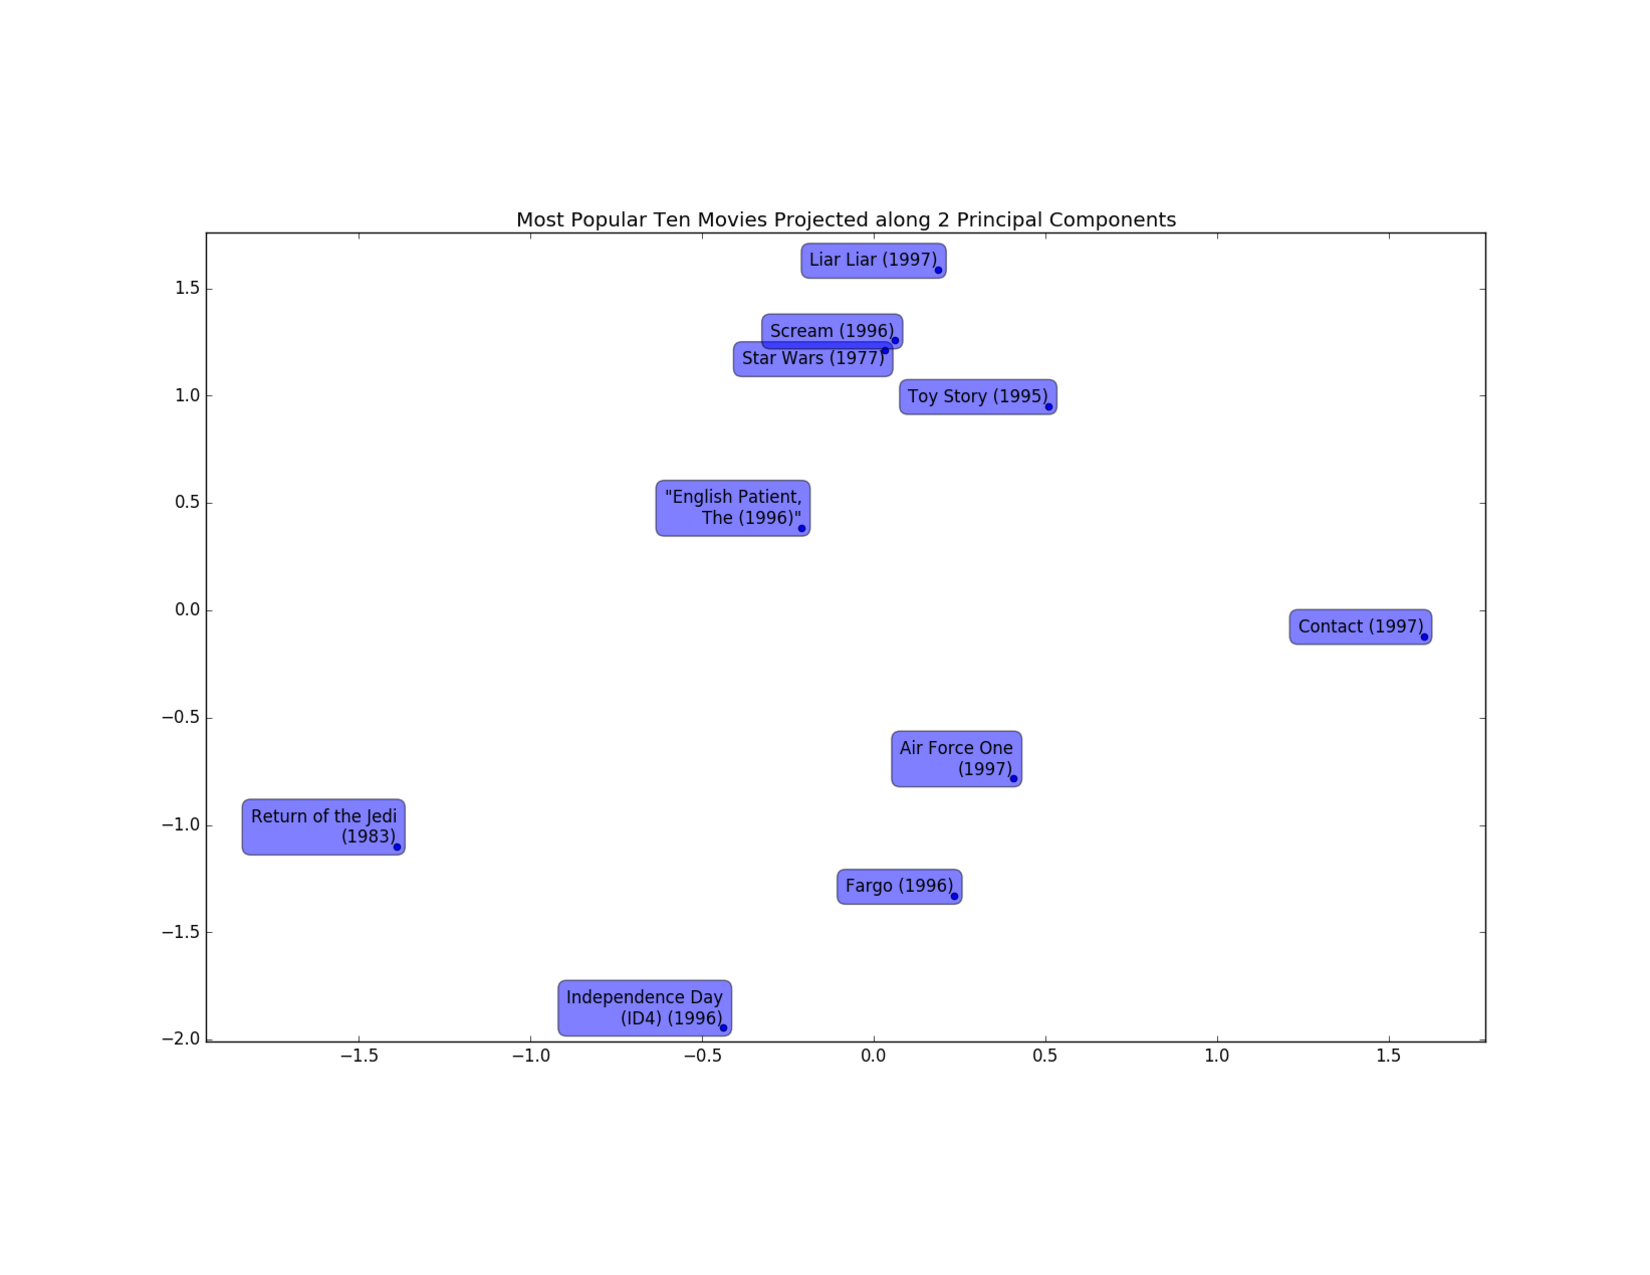
\includegraphics[width=0.8\textwidth, angle =270]{Popular_10_Movies.pdf}
 \caption{Most popular ten movies projected along two principal components.}
\label{fig:tenMostPopular}
\end{figure}


\begin{figure}[hptb]
\centering
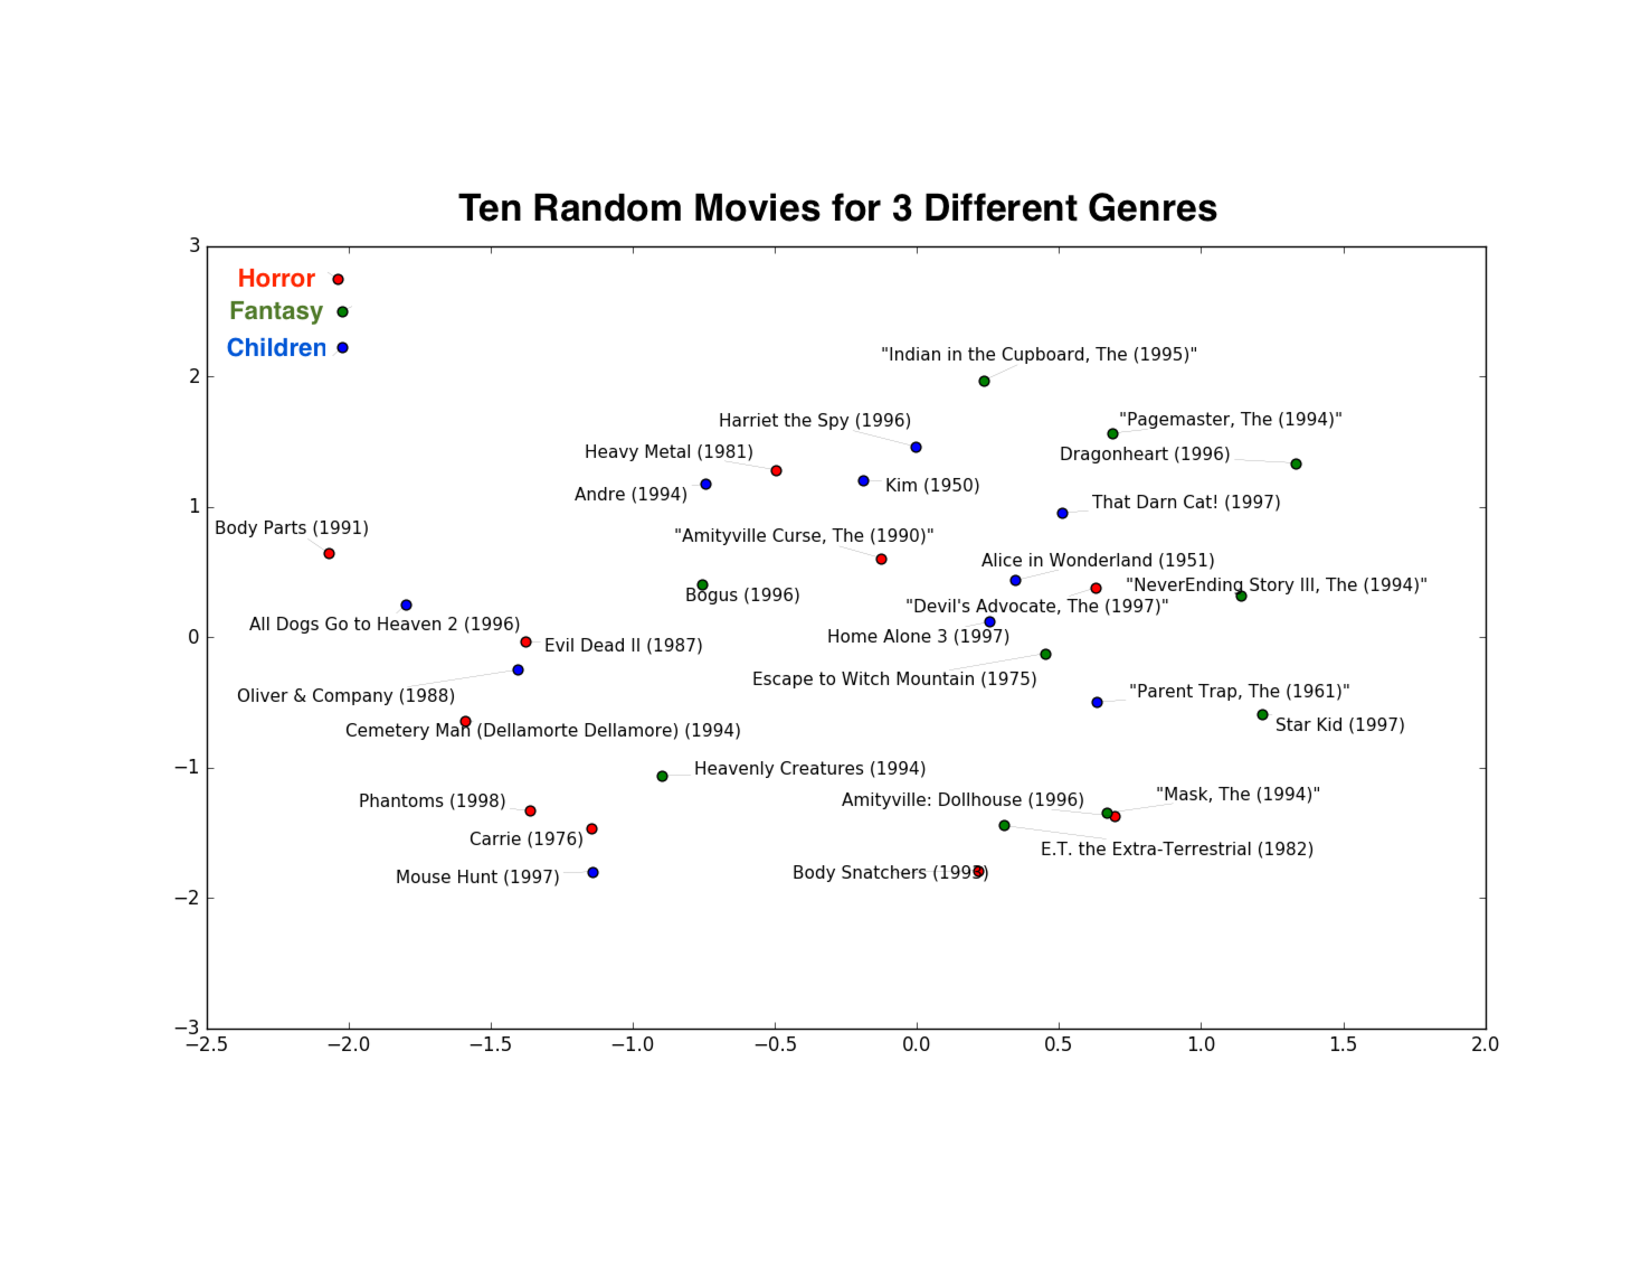
\includegraphics[width=0.8\textwidth, angle =270]{Three_Genres.pdf}
 \caption{ }
\label{fig:tg}
\end{figure}

\section{Conclusion}

From our analysis, we were able to visualize movies along the top 2 principal components which capture the most variance in movie ratings. However, from our visualization plots, there seems to be little human-understandable correlation between movies that are close together in the 2 principal component dimensions. To us, it seemed that many movies that were quite different to each other ended up close together in the 2D visualization. 

Furthermore, when looking at the mean movie coordinates for each genre, it at first suggested a correlation between genre and position along the principal components (e.g. Documentary and Children are far from each other in the Principal Component space). However, when we look at the standard deviation among each genre along both the x-axis and y-axis, this correlation becomes quite unreliable as the variance for each genre is so high. 

It seems then that the meaning of each principal component is not easily human-understandable. Our best hypothesis is that the first principal component (x-axis) is correlated with the skewness of the average movie rating distribution, such that large x-values indicate that the rating distribution skews left and vice versa.

\end{document}
